Extracting knowledge from a developed system can provide potential benefits for searching, browsing, and discovering them among a huge set of software systems.
\GH is one of the most used developing service that includes version control systems (\ie git) plus social and collaborative features (\eg bug tracking, contribution requests, task management, and wikis).
At the moment we are writing this contribution, \GH counts more than 40 million users and over 100 million repositories. Because of this huge among of data, the availability of reusable projects might be compromised if they cannot be suitably discovered. In recent years, \GH introduced a topic mechanism to explore repositories in a particular subject area, learn more about that subject, and find projects to contribute to.
\GH continuously monitors the stored repository and assigned topics to organize the former with respect to the list of assigned topics. Moreover, those data are periodically analysed to extract the most popular and active topics (\ie \emph{featured topics\footnote{\url{https://github.com/topics}}}). Thus, users can monitor the community’s trend by consulting such a public list. In the beginning, this activity was entirely done by humans (\ie project contributors) that label the repository according to their knowledge, feeling and belief. Literature is plenty of several approaches that mine and exploit available data to analyze repositories. Nevertheless, few of them cope with the topic recommendation task, which can be crucial in the project's development initial phase. Figure \ref{fig:SpaceshipGenerator} shows an example repository with related topics. By this simple snapshot, a \GH user can figure out that the \emph{SpaceshipGenerator}\footnote{\label{note:spaceship}\url{https://github.com/a1studmuffin/SpaceshipGenerator}} project makes usage of \emph{Blender-scripts} (\ie a \emph{python} 3d modeling library) for \emph{procedural-generation} of \emph{3d} spaceships from a random seed.


%analyze \emph{big-data} and databases by exploiting common techniques used in this domain \ie \emph{sql and jdbc}. 

\begin{figure}[h!]
	\centering
	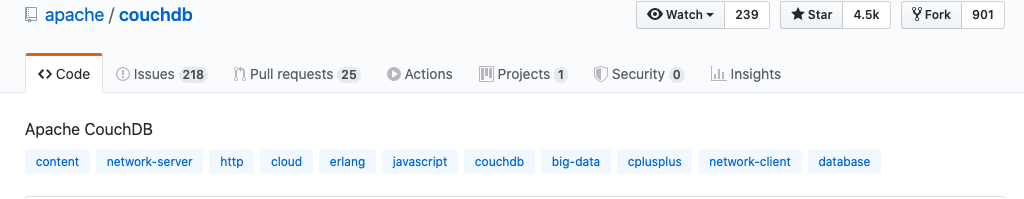
\includegraphics[width=0.99\linewidth]{figs/SpaceshipGenerator.png}
	\caption{A \GH repository with different topics.}
	\label{fig:SpaceshipGenerator}
\end{figure}


As mentioned before, the \MNB using the \RM file of a repository to predict featured topics. It involves all the standard techniques employed in the ML domain \ie textual engineering, feature extraction, and training phase. By relying on the multinomial probability distribution, the approach is able to extract relevant information from the \RM file and suggest a set of topics. Table \ref{tab:example} shows an example of the \MNB's outcomes given the list of the actual repository topics. 

\begin{table}[h]
\centering

\resizebox{8.5cm}{!} {

\begin{tabular}{| p{3.2cm} | p{3.2cm} | }
\hline
 \textbf{Actual Topics} &\textbf{ Predicted topics} \\ \hline
     python,blender-scripts, spaceship, procedural-generation, game-development, 3d        &  
  shell, terminal, \textbf{3d},	opengl,	\textbf{python}        \\ \hline

\end{tabular}
}
\caption{Example of the \MNB outcomes for \emph{SpaceshipGenerator} repository.}
\label{tab:example}
\end{table} 



Even though the \MNB works in practice, it suffers from some limitations. First, the underlying model can recommend only featured topics that represent only a small set of all possible terms that can be restricted because of antonymous term(\eg programming languages).

For instance, \emph{blender-scripts}\footnote{blender is the most used python library to manipulate 3d objects. \url{}https://www.blender.org/} as well as \emph{game-development} could be recommended as possible topics because the project includes both \emph{3d} and \emph{python} topics.
In this way, the \MNB doesn't express all the concepts covered by a \GH repository. As shown in the table, only two of the predicted topics matched with the real ones. Moreover, in the case the repository already includes all suggested topics, \MNB does not able to recommend new ones.
The second major limitation is the underlying structure needed for the training phase. To deliver relevant items, the \MNB requires a \emph{balanced} dataset, \ie each topic must have a similar number of  \RM files. This is hard to come by in practice as topics are generally heterogeneous.
%This scenario is difficult to meet in reality as the topics' heterogeneity is extremely high. 
Furthermore, repositories in \GH are regularly updated with new new topics and thus, the training phase must take place several times to avoid outdated recommendations. 

In the recent years, many techniques have been conceived to predict interest a of an user by relying on the preferences collected from other users. Such techniques can be classified as  \emph{content-based}~\cite{Pazzani2007} where the relationships among items have been exploited to predict the most similar items,
or \emph{collaborative-filtering}~\cite{Miranda:2008:ICF:1486927.1487083} that calculates the missing ratings by taking into account the set of items rated by similar customers. There are two main types of collaborative-filtering recommendation: \emph{user-based} \cite{Zhao:2010:UCR:1748610.1749278} and \emph{item-based} \cite{Sarwar:2001:ICF:371920.372071} techniques. The former computes missing ratings by considering the ratings collected from similar users, whereas, the latter performs the same task by using the similarities among items \cite{Cremonesi:2008:EMC:1468165.1468327}.